\documentclass{article}

\usepackage{graphicx}
\usepackage{amsmath}
\usepackage{caption}
\usepackage{subcaption}
\usepackage{listings}
\usepackage[hidelinks]{hyperref}
\usepackage{enumitem}
\usepackage{geometry}

\renewcommand{\contentsname}{Table of Contents}

\begin{document}

\begin{titlepage}
\begin{center}
\vspace*{1cm}

\Huge
\textbf{Project 01: Home Safe}

\vspace{0.5cm}
\Large
\textit{Requirements Definition Document} \\
\textit{RDD Version 1.0}

\vspace{1cm}

\textbf{Team 01}

\vspace{0.5cm}

\text{Marina Seheon (Manager)} \\
\text{Andrei Phelps (Document Manager)} \\
\text{Luke McDougall} \\
\text{Jack Vanlyssel} \\
\text{Spoorthi Menta} \\
\text{Vamsi Krishna Singara} \\

\vspace{1cm}

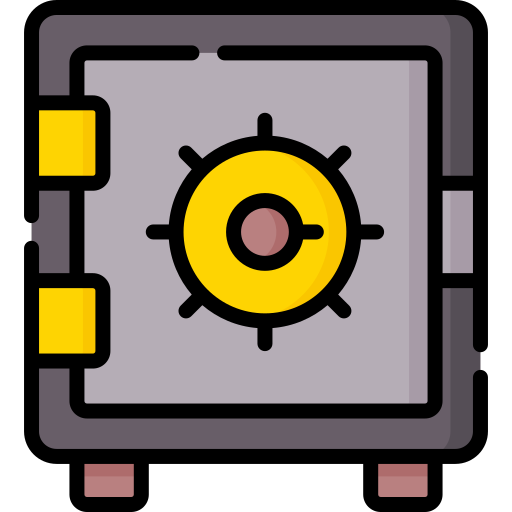
\includegraphics[scale=0.25]{docs/figs/safe.png}\\[0.5cm]

\vspace{3.5cm}

\Large
\textbf{CS460: Software Engineering} \\

\end{center}
\end{titlepage}

\newpage

\tableofcontents

\newpage

\section{Introduction}
Contained herein are the specific requirements for HomeSafe, our innovative new safe built from the ground up with convenience and security in mind. While traditional lock safes have served their purpose in many households, the surge in demand for digital safes among Americans is a result of their enhanced convenience and security. HomeSafe is poised to redefine conventions by offering an unparalleled fusion of security and convenience. This goal will be achieved through the integration of cutting-edge biometric technology, including a retina scanner, seamlessly woven into its two-factor authentication mechanism. Significantly, during the development phase, we actively collaborated with our marketing team to ensure that HomeSafe's features aligned with market expectations and preferences. \\ \\
A notable feature that distinguishes HomeSafe is its ability to accommodate multiple users seamlessly, making it a versatile solution. Moreover, our design prioritizes ease of maintenance and setup. The user-friendly interface ensures that HomeSafe can be effortlessly managed and configured, allowing for a hassle-free experience for both administrators and individual users. This innovation is well-suited for household consumers committed to reinforcing the protection of their assets, including money, jewelry, critical documents, and treasured possessions.

\section{Definition of Terms}
Within this section, we provide definitions for key terms that are recurrently utilized throughout the document. This section can serve as a point of reference for readers as they engage with the content.

\begin{enumerate}
    \item[I.] \textbf{Administrator}: An individual with the authority to establish and oversee separate user profiles within the system, regulating user access to the system's settings and contents.
    \item[II.] \textbf{Auxiliary}: An additional or secondary power source that supports the main or primary power supply. An auxiliary power source is typically used to provide backup, redundancy, or temporary power in situations where the main power source is unavailable, disrupted, or insufficient.
    \item[III.] \textbf{Bio-Metric Scanner}: A technology that identifies and authenticates users based on their unique biological characteristics, typically fingerprints, retina patterns, or other distinct traits.
    \item[IV.] \textbf{Microcontroller}: A microcontroller is a small integrated circuit serving as the central processing unit (CPU) of a safe's electronic system. It contains a processor, memory, and input/output ports and can include programmable capabilities. Microcontrollers manage tasks, user input, security protocols, and control functions in the safe, including locks, interface interactions, and external device communication.
    \item[V.] \textbf{Personal Identification Number (PIN)}: A numerical code that serves as a security credential used to authenticate and verify the identity of an individual. PINs are commonly used in various systems, such as electronic devices, bank accounts, and access control systems, to ensure that only authorized users can gain access.
    \item[VI.] \textbf{Two-Factor Authentication (2FA)}: A security protocol that requires users to provide two distinct forms of verification to access a system. This commonly involves a combination of something known (such as a password) and something possessed (such as a generated code or biometric information), adding an extra layer of security and protection against unauthorized access.
\end{enumerate}

\section{Objectives}
Our primary aim is to create a platform within our safe that accommodates multiple individual users, granting independent access while allowing the administrator to extend access to up to five users. Simplicity of setup and maintenance has been a core objective, reflected in the user-friendly interface that ensures easy management and configuration. This convenience extends to the activation of Two-Factor Authentication, bolstering security with a biometric retina scan. This security-focused approach maintains user data integrity even during power outages, underscoring our commitment to seamless access and protection.

\subsection{Multi-User Capability}
The safe will include the functionality to store codes for numerous users. The administrator has the authority to provide access to as many as (insert number here) distinct users. Each user will have the capability to unlock the safe. Additionally, the administrator can monitor the opening and closing of the safe, recording details about who accessed it and when it was shut.

\subsection{Enhanced Security with Two-Factor Authentication}
To enhance security measures, users can opt for Two-Factor Authentication (2FA). This involves receiving a code through their chosen 2FA method, such as biometric retina scans, which are then inputted into the safe to finalize setup. Once activated, users are required to enter the 2FA code alongside their individual safe code to gain access, ensuring an added layer of protection.

\subsection{Easy Setup and Care}

When you receive HomeSafe, the setup process is made smoother with pre-installed batteries, eliminating the requirement for extra assembly. The unit is meticulously designed for user-friendly operation: just power on the safe and follow the straightforward prompts to finalize the setup. This method guarantees a seamless experience right from the beginning, reducing user involvement and erasing the usual intricacies linked to initial installation.

\subsection{Uninterrupted Security and Access}
Should a power failure occur, rest assured that the safe retains its stored user data intact. However, for users who have activated 2FA, accessing the safe will necessitate the presence of the administrator to grant access in the absence of regular authentication. This safety measure underscores our commitment to maintaining data integrity and security, even during unexpected power interruptions.

\section{System Organization}
In this section, we offer an outline of the organizational structure of the HomeSafe system, encompassing insights into its user interface, as well as its internal components and their interplay.

\subsection{User Interface}
This section will provide an overview of the user interface. The user will utilize a keypad with numbers 0-9, volume buttons, a * key, a red x key, a green circle key, an iris scanner, an LED display, a speaker, and a door handle.

\vspace{0.3cm}

\begin{center}
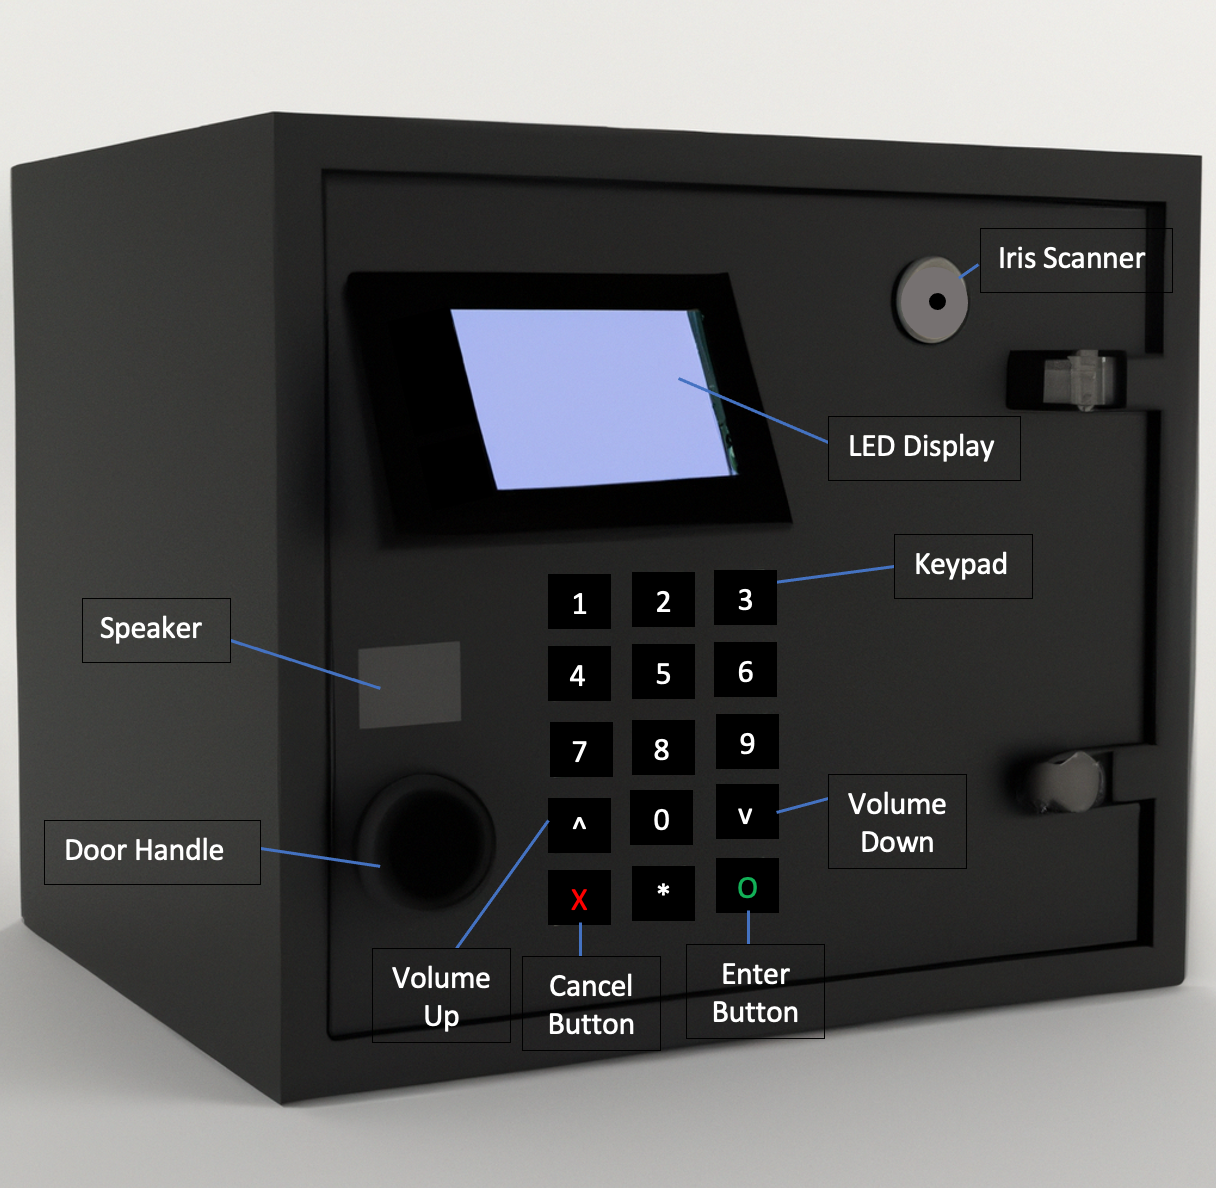
\includegraphics[scale=0.7]{docs/figs/safe_image1.png}
\end{center}

\begin{enumerate}
    \item \textbf{Keypad}: The secondary source of authentication. Once the bio-metric scan is complete, the user must input their six-digit PIN using the number keys labeled 0-9, along with a * character. If the user enters an incorrect PIN or lets more than three seconds elapse after input, the system will reset the user's attempt. After three failed attempts, the user will be restricted access and will need an administrator's PIN to regain access.
    \item \textbf{Red X Key}: If a user makes an incorrect entry during PIN entry, they can press this button to reset their attempt. This will not be counted as a failed attempt.
    \item \textbf{Green Circle Key}: The user must press this button after all six digits of their PIN have been entered. Upon pressing this button and entering the correct PIN, the latches will be released, allowing the user access.
    \item \textbf{LED Display}: The display screen serves as the communication medium with the user. When a password is entered, the display indicates the number of keys that have been input. This functionality is incorporated to improve user convenience.
    \item \textbf{Iris Scanner}: The primary source of authentication. Once the user provides a retinal scan, the microcontroller will enable communication with the keypad. This will send a prompt for the user to input their six-digit code using the keypad on the LED Display.
    \item \textbf{Speaker}: Provides auditory feedback to the user when interacting with the user interface.
    \item \textbf{Volume Buttons}: Allows the user to increase or decrease volume levels.
    \item \textbf{Door Handle}: Used to open the safe once the latches have been released after successful authentication.
\end{enumerate}

\subsection{Interior Design}
In this section, we outline how the internal components of HomeSafe are organized. These components encompass the safe materials, the locking system, and the elements responsible for governing HomeSafe's software and power management.

\begin{enumerate}
    \item \textbf{Foam Interior Base}: A soft foam base that covers the steel floor of the safe. This allows for the safe storage of otherwise delicate items.
    \item \textbf{Steel Latches}: While the safe is in a locked state, the twin steel latches will press down on the lock sensors.
    \item \textbf{Lock Sensors}: Communicates with the microcontroller whether the safe is in the locked or unlocked state.
    \item \textbf{Micro-Controller}: Powered by the batteries, this is where the brains of the system are housed. Inputs are received and interpreted prior to sending any kind of output to the user. Requires power to store user data such as PINs, bio-metric, and user data.
    \item \textbf{Battery Compartment}: Compartment where the primary power source, two AA batteries, is stored.
    \item \textbf{Auxiliary Power}: The secondary power source is stored inside the microcontroller, a single CR2032 cell battery.
\end{enumerate}

\section{Capabilities}
The safe's design incorporates a diverse range of functionalities, all of which align seamlessly with the established project objectives. These stipulated capabilities collectively guarantee that HomeSafe retains its user-friendly interface, heightened security measures, and uninterrupted security and access even in the event of power failures. The subsequent sections expound upon these meticulously discussed features to provide a comprehensive understanding of their implementation within HomeSafe's framework.

\subsection{Multi-User Capability}
The Multi-User Capability enhances convenience and swift access for numerous individuals, promoting seamless collaboration. This feature includes:

\begin{itemize}
    \item \textbf{User Profiles}: Create and manage distinct user profiles within the system, each with its own access permissions and settings.
    \item \textbf{Customized Access Levels}: Assign different access levels to users, allowing them to interact with specific functions or data based on their roles.
    \item \textbf{Multi-User History}: Maintain a log of actions performed by different users for accountability and monitoring purposes.
    \item \textbf{Access Time Windows}: Define specific time periods during which certain users are allowed access, enhancing control over usage.
    \item \textbf{Revocation of Access}: Enable primary users to revoke access for secondary users when necessary.
\end{itemize}

\subsection{Enhanced Security with Two-Factor Authentication}
Attain elevated security and a deep sense of peace of mind through Two-Factor Authentication, encompassing the following fundamental elements:

\begin{itemize}
    \item \textbf{Advanced Security}: Implementation of two-factor authentication significantly fortifies security measures, ensuring unauthorized access is thwarted.
    \item \textbf{Comprehensive Access Control}: Incorporating multiple verification factors allows for more comprehensive control over who can access the system.
    \item \textbf{Reduced Vulnerability}: Enhanced security through 2FA translates to a reduced vulnerability to hacking, phishing, and other malicious activities.
\end{itemize}

\subsection{Easy Setup and Care}
This robust set of features ensures the system's reliability, ease of use, and continual security, aligning perfectly with the goal of efficient, user-friendly operation.

\begin{itemize}
    \item \textbf{Hassle-Free Setup}: The unit is delivered with batteries already installed, eliminating the need for consumers to set up the batteries themselves. It operates exclusively on battery power, eliminating the necessity for an AC power source.
    \item \textbf{Intuitive Interface}: Design a user-friendly interface that guides users through the setup process effortlessly.
    \item \textbf{Automatic PIN Renewal}: The system intelligently prompts users to change their PIN every six months, bolstering security measures proactively.
\end{itemize}

\subsection{Uninterrupted Security and Access}
Strengthening seamless security and access, these integrated features form the cornerstone of sustained operational reliability, bolstering the system's trustworthiness across various circumstances.

\begin{itemize}
    \item \textbf{Backup Power Integration}: Integrated auxiliary power source that seamlessly takes over when the main battery depletes.
    \item \textbf{Advanced Low-Battery Alerts}: DProvide early notifications to users when the battery level is dropping, enabling them to take proactive measures.
    \item \textbf{Emergency Power Reserve}: Designate a portion of the battery capacity as an emergency reserve, ensuring critical operations can continue even if the battery is almost depleted.
\end{itemize}

\section{Design Constraints}
The HomeSafe design adheres to the following usage and physical limitations within the system.

\begin{itemize}
    \item For standard operation, two functioning AA batteries must be inserted into the unit. In the event one or more of these batteries dies, the unit will automatically switch to an auxiliary power supply located in the microcontroller, which is a single CR2032 battery.
    \item The auxiliary power supply can power the system for approximately 5-8 years. If the auxiliary power supply is depleted before the primary power supply is restored, all user data will be lost and the contents of the unit will not be accessible.
    \item If a user without administrative access loses access to their PIN, they will be completely unable to access the HomeSafe. An administrator must grant access to the specific user to reset a PIN.
    \item The HomeSafe is 12 x 16 x 12 inches (L x W x H). This may limit how much the customer is able to store inside.
\end{itemize}

\section{References}
The websites and other sources we used to gather images and information.

\begin{enumerate}
    \item “Dall·E 2.” DALL·E 2, openai.com/dall-e-2. Accessed 28 Aug. 2023.
    \item “Everything You Need to Know about the CR2032 Battery.” Microbattery, Microbattery.com, 8 Mar. 2023, www.microbattery.com/blog/post/battery-bios:-everything-you-need-to-know-about-the-cr2032-battery/.
    \item Garska, Kathleen. “Two-Factor Authentication (2FA) Explained: Biometric Authentication.” Identity Automation Blog, blog.identityautomation.com/mfa-face-off-series-biometric-authentication. Accessed 28 Aug. 2023.
    \item Lutkevich, Ben. “What Is a Microcontroller and How Does It Work?” IoT Agenda, TechTarget, 7 Nov. 2019, www.techtarget.com/iotagenda/definition/microcontroller.
    \item “Safe Icons.” Flaticon, www.flaticon.com/search?word=safe. Accessed 25 Aug. 2023.
\end{enumerate}

{\parindent0pt}

\end{document}
